\section{Computational performance}
\label{sec:performance}

The tensor formulation exposes the independent SURF columns to batched
accelerator execution without changing the prognostic calculation. We
measured the autonomous offline implementation against the Fortran reference
over progressively larger subsets of the effective 2018 CMFD domain. Each run
used the same restart, forcing representation, double-precision state and
arithmetic, and 1800~s physics step as
Sect.~\ref{sec:annual-autonomous-equivalence}. A timed segment contains 240
continuous steps (5 simulated days). The Fortran reference was timed with
\texttt{osmMASTER} under 32 OpenMP threads on an Intel Xeon Gold 6430 host;
the accelerator experiments use one NVIDIA A100 80~GB GPU. Each configuration
was run independently three times and the median is reported. All timing runs
use the pinned software environment of
Sect.~\ref{sec:annual-autonomous-equivalence}.

The timing boundary is deliberately narrow. State output is disabled, the
optional per-step host-side non-finite check is disabled, and the GPU stream
is synchronized immediately after the final model step. The final state is
then checked for finite values outside the timed interval. Consequently,
integration time measures the continuous physics calculation rather than
initial-state loading, diagnostic transfer, file serialization, or the
one-time forcing load; the Fortran timing is the internal time-step-loop
section, excluding initialization, forcing reads, and restart I/O.

Two accelerator configurations are reported. The eager configuration launches
each tensor operation individually; the CUDA-graph configuration records one
complete physics step (forcing construction plus the full model update) into
a single replayable graph, so subsequent steps launch once. Making the step
capturable required eliminating every host synchronization in the step: scalar
reads of device tensors were replaced by broadcast views, per-step host-side
constant materializations were cached on the device, and the one
state-dependent host branch was replaced by an idempotent masked update. Each
change is bit-identical to the eager path, and the captured integration
reproduces the eager trajectory bit for bit at 1,000 and at 97,709 columns.

\begin{table}[t]
\caption{Batch-size performance of the double-precision autonomous offline
SURF integration against the Fortran reference on the same columns. Values
are median wall-clock integration times in seconds (parentheses give the
minimum--maximum range across three repeats). Each integration contains 240
continuous 1800~s steps. The rightmost columns give each accelerator
configuration's speed-up over the 32-thread Fortran reference.}
\label{tab:performance-scaling}
\centering
\small
\begin{tabular}{rrrrrr}
\hline
Active & Fortran & Torch A100 & Torch A100 & \multicolumn{2}{c}{speed-up over Fortran} \\
columns & 32 threads (s) & eager (s) & graph (s) & eager & graph \\
\hline
1,000 & $0.55$ ($0.53$--$0.61$) & $16.98$ ($16.32$--$17.71$) & $4.60$ ($4.59$--$4.63$) & $0.03\times$ & $0.12\times$ \\
10,000 & $8.29$ ($8.27$--$8.66$) & $15.81$ ($15.39$--$16.11$) & $5.09$ ($5.09$--$5.13$) & $0.52\times$ & $1.63\times$ \\
50,000 & $28.26$ ($28.14$--$28.68$) & $14.87$ ($14.62$--$14.98$) & $8.37$ ($8.35$--$8.43$) & $1.90\times$ & $3.38\times$ \\
97,709 & $53.38$ ($49.60$--$53.57$) & $18.13$ ($18.12$--$18.67$) & $13.90$ ($13.81$--$13.93$) & $2.94\times$ & $3.84\times$ \\
\hline
\end{tabular}
\end{table}

Figure~\ref{fig:performance-scaling} shows the three configurations. The
Fortran reference is the most efficient configuration below about ten
thousand columns, where per-step kernel-launch overhead dominates the Torch
integrations: the step issues thousands of small CUDA kernels, and at small
batches their launch latency exceeds the computation they carry. Recording
the step once and replaying it removes that floor: the graph configuration
outperforms the Fortran reference from about eight thousand columns upward,
and reaches $3.84\times$ over the complete effective domain. For the complete
effective CMFD domain, the graph configuration reaches
$1.69\times10^{6}$ column-steps~s$^{-1}$, compared with
$4.39\times10^{5}$ column-steps~s$^{-1}$ for the Fortran reference. The gain
comes from batched evaluation of the same 1800~s double-precision process
sequence, rather than from an altered time step or forcing representation.

\begin{figure}[t]
\centering
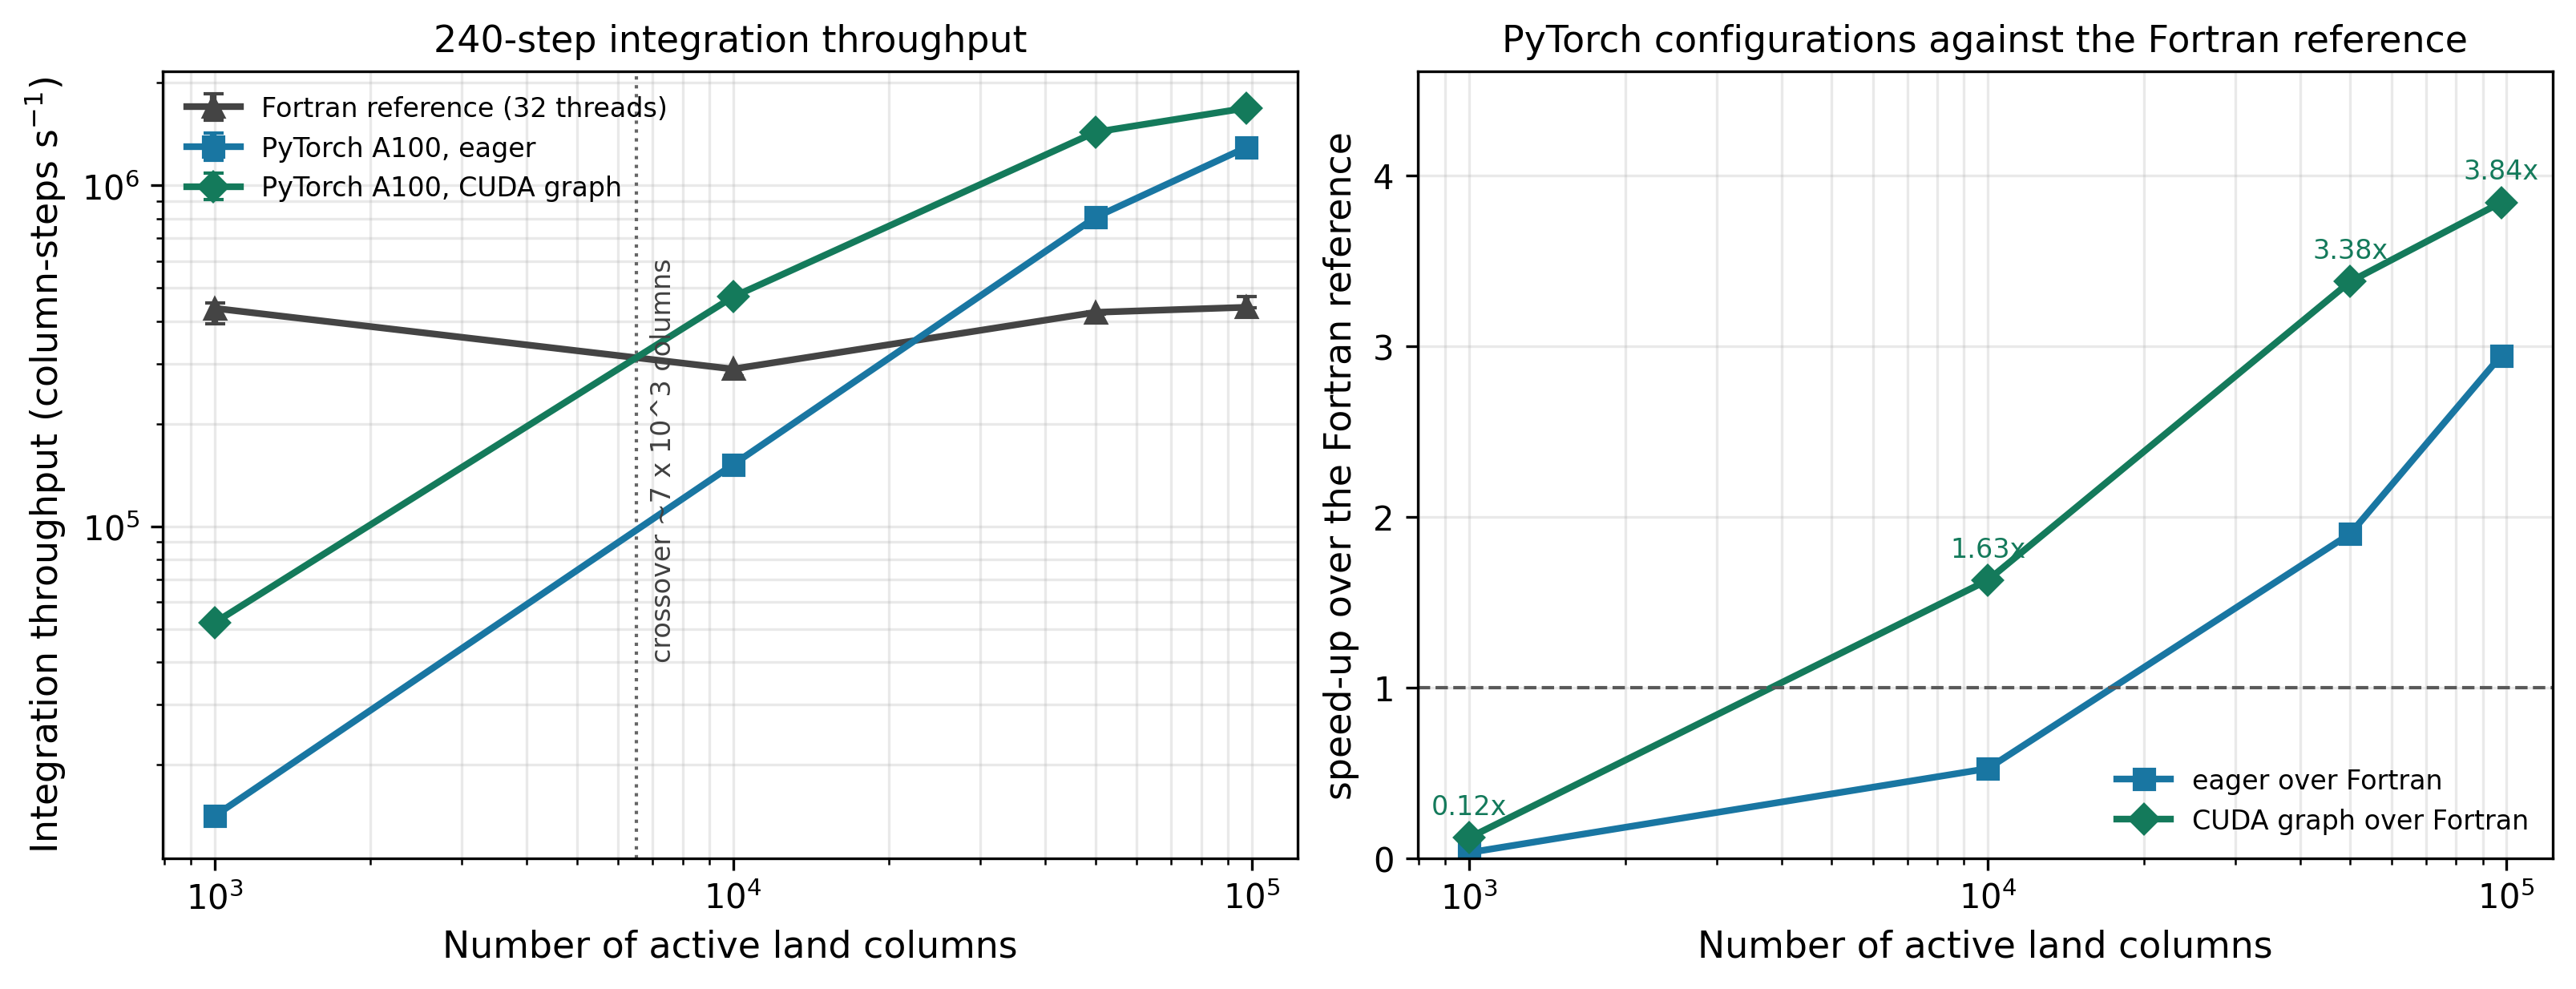
\includegraphics[width=\linewidth]{figures/surf_fortran_graph_scaling.png}
\caption{Integration throughput and accelerator speed-up for the autonomous
offline SURF implementation over 240 continuous steps, against the Fortran
reference on the same columns. Left: throughput for the Fortran reference and
the A100 eager and CUDA-graph configurations; points are repeat medians,
error bars span the observed minimum--maximum integration times. Right: each
accelerator configuration's speed-up over the Fortran reference.}
\label{fig:performance-scaling}
\end{figure}

These gains are in line with published ports of comparable double-precision
physics. The GT4Py rewrite of the FV3 dynamical core reports
$3.3\times$ over its optimized Fortran reference on float64
\citep{Dahm2023Pace}; a JAX port of the multilayer-canopy CLM-ml reports
$2.2\times$--$4.7\times$ over sequential Fortran, with no benefit from single
precision on this bandwidth-bound class of code \citep{Lahlou2026CLMml}; and
the full OpenACC port of ICON reports $5.5\times$ socket-to-socket for the
complete model \citep{Lapillonne2026ICON}. CUDA-graph recording of small
soil and turbulence kernels in the ICON port translated to about 5~\%
end-to-end; the larger gain here follows from the unusually high kernel count
per step of the tiled column physics. Double-digit GPU-versus-CPU claims in
this literature trace to unoptimized CPU baselines or many-GPU against
single-CPU-node comparisons, and are not the like-for-like regime measured
here.
